\begin{frame}[fragile]{Grafer}
    Veldig mange algoritmeproblemer kan representeres som grafer.
    \begin{columns}
        \begin{column}{0.3\textwidth}
            \begin{figure}
                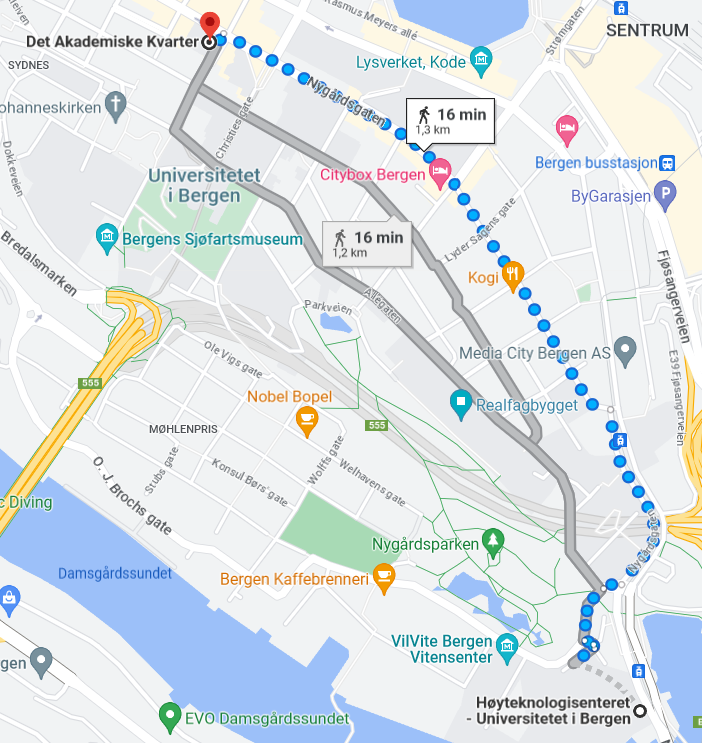
\includegraphics[width=4cm]{images/Kvarteret.png}
                \caption{Hva er kjappeste veien til Kvarteret?}
            \end{figure}
        \end{column}
        \begin{column}{0.3\textwidth}
            \begin{figure}
                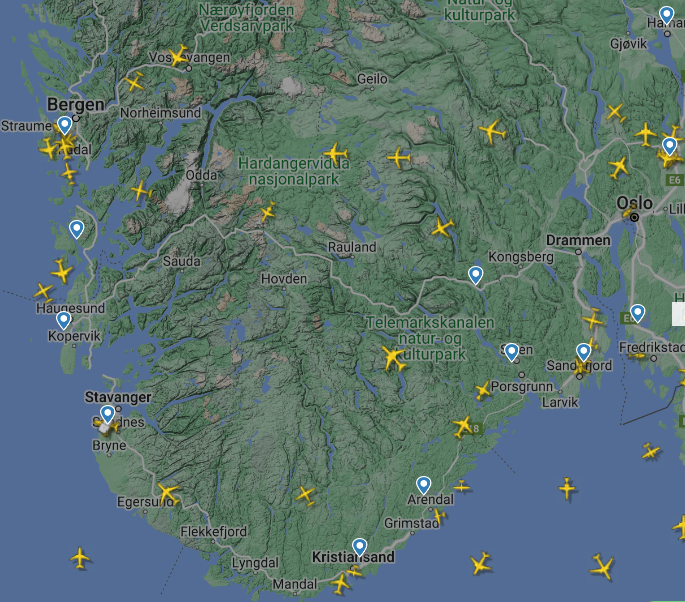
\includegraphics[width=4cm]{images/Bergen.png}
                \caption{Hvilke fly kan du ta for å komme deg hjem fortest?}
            \end{figure}
        \end{column}
        \begin{column}{0.3\textwidth}
            \begin{tikzcd}
                                  & b \arrow[rr, no head] &                                           & e \arrow[loop, distance=2em, in=305, out=235] \\
            a \arrow[rr, no head] &                       & d \arrow[lu, no head] \arrow[ld, no head] &                                               \\
                                  & c \arrow[lu, no head] &                                           &                                              
            \end{tikzcd}
        \end{column}
    \end{columns}
\end{frame}


\subsection*{Begreper}
\begin{frame}
    \begin{block}{Graf $G(V,E)$}
    En Graf $G = (V, E)$ er et sett noder (vertices) $V$ og et sett kanter (edges) $E$.
    \end{block}
    \pause

\begin{columns}
    \begin{column}{0.28\textwidth}
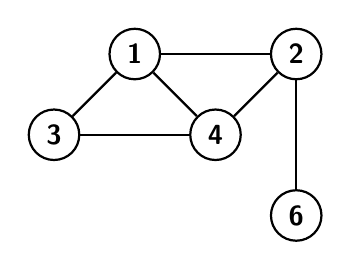
\begin{tikzpicture}[
    node distance=1.45cm, thick,
    main node/.style={circle, draw, font=\sffamily\bfseries}
]
    \node[main node] (1)                    {1};
    \node[main node] (3) [below left  of=1] {3};
    \node[main node] (4) [below right of=1] {4};
    \node[main node] (2) [above right of=4] {2};
    \node[main node] (6) [below right of=4] {6}; % <-4> forces an additional overlay in which node 2 disappears

    \path (1) edge (2)
        (4) edge (2)
        (6) edge (2);
    \path (1) edge (3)
        (4) edge (1);
    \path (3) edge (4);
\end{tikzpicture}
 \end{column}
 \pause
    \begin{column}{0.68\textwidth}
\begin{itemize}[<+->]
    \item Noder: $V=\{1,2,3,4,6\}$ \pause
    \item Kanter: $E=\{(1,2), (1,4), (3,4), (2,4), (2,6), (1,3)\}$\pause
    \item Sti (/path): Vei fra A til B\\
    Eksempel: $Path(1,6)=[1,2,6]$\pause
    \item Sykel (/Cycle): En sti med samme start og slutt\\
    Eksempel: $[1,3,4,1]$, $[1,2,4,3,1]$\pause
    \item Nabolag: Alle naboene en node kan nå med én kant\\
    Eksempel: $N(4)=\{1,2,3\}$, $N(6)=\{2\}$\pause
    \item Grad (/degree): Antall naboer av en node\\
    Eksempel: $deg(4)=3$, $deg(6)=1$
\end{itemize}
 \end{column}
\end{columns}
\end{frame}

\begin{frame}{Rettede grafer}
    Om du skal lage en graf av veinettverket i Bergen, får du fort problemer. Hele sentrum er jo enveiskjørt! Vi trenger å kunne representere enveiskanter.
    \begin{columns}
    \begin{column}{0.475\textwidth}
    \begin{figure}
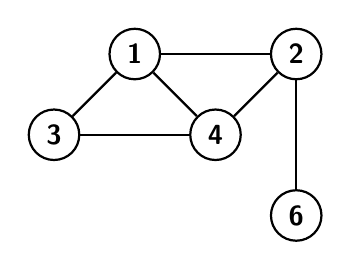
\begin{tikzpicture}[
    node distance=1.45cm, thick,
    main node/.style={circle, draw, font=\sffamily\bfseries}
]
    \node[main node] (1)                    {1};
    \node[main node] (3) [below left  of=1] {3};
    \node[main node] (4) [below right of=1] {4};
    \node[main node] (2) [above right of=4] {2};
    \node[main node] (6) [below right of=4] {6}; % <-4> forces an additional overlay in which node 2 disappears

    \path (1) edge (2)
        (4) edge (2)
        (6) edge (2);
    \path (1) edge (3)
        (4) edge (1);
    \path (3) edge (4);
\end{tikzpicture}
\caption{Urettet graf (undirected).\\$deg(4) = 3, N(4) = [1, 2, 3]$}
\end{figure}
 \end{column}
 \pause
    \begin{column}{0.475\textwidth}
    \begin{figure}
    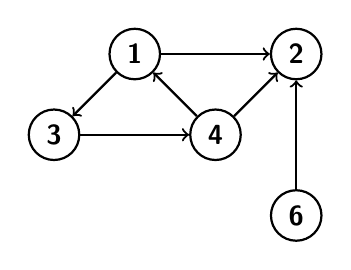
\begin{tikzpicture}[
    node distance=1.45cm, thick,
    main node/.style={circle, draw, font=\sffamily\bfseries}
]
    \node[main node] (1)                    {1};
    \node[main node] (3) [below left  of=1] {3};
    \node[main node] (4) [below right of=1] {4};
    \node[main node] (2) [above right of=4] {2};
    \node[main node] (6) [below right of=4] {6}; % <-4> forces an additional overlay in which node 2 disappears

    \path[->] (1) edge (2)
        (4) edge (2)
        (6) edge (2);
    \path[->] (1) edge (3)
        (4) edge (1);
    \path[->] (3) edge (4);
\end{tikzpicture}
\caption{
    Rettet graf (directed).\\
    $deg^+(4) = deg^{out}(4) = 2$\\
    $deg^-(4) = deg^{in}(4) = 1$\\
    $N^+(4) = N^{out}(4) = [1, 2]$\\
    $N^-(4) = N^{in}(4) = [3]$
}
\end{figure}
 \end{column}
\end{columns}
\end{frame}

\begin{frame}
    \begin{block}{Bipartitte grafer $G(V,A,B)$}
    En bipartitt graf er en graf som kan deles i to sett $A,B$ der alle kanter $v\in V$ går fra en node i $A$ til en node i $B$. Grafen kan fargelegges i to farger slik at alle kanter går fra én farge til en annen farge.
    \end{block}

\begin{tikzpicture}[
    node distance=1.45cm, thick,
    main node/.style={circle, draw, font=\sffamily\bfseries}
]
    \node[main node,onslide=<2->{fill=black!40!green}] (1)                    {1};
    \node[main node,onslide=<2->{fill=black!40!green}] (3) [below left  of=1] {3};
    \node[main node,onslide=<2->{fill=black!40!green}] (4) [below right of=1] {4};
    \node[main node,onslide=<2->{fill=black!30!red}] (2) [above right of=4] {2};
    \node[main node,onslide=<2->{fill=black!30!red}] (5) [below right of=3] {5};
    \node[main node,onslide=<2->{fill=black!30!red}] (6) [below right of=4] {6};

    \path (1) edge (2)
        (1) edge (5)
        (3) edge (5)
        (4) edge (2)
        (4) edge (5)
        (4) edge (6);
\end{tikzpicture}
\end{frame}

\begin{frame}{Trær}
    \begin{itemize}
        \item Et \emph{tre} er en \textit{sammenhengende}, \textit{urettet} graf uten sykler.
        \item En \emph{skog} er en graf med flere trær som ikke er tilknyttet hverandre.
        \item Et \emph{blad} i et tre er en node som har grad 1.
        \item En \emph{intern node} i et tre er en node som ikke er et blad.
    \end{itemize}
    \begin{columns}
    \begin{column}{0.48\textwidth}
\begin{figure}
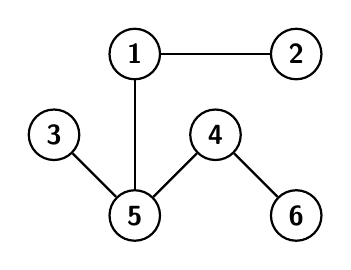
\begin{tikzpicture}[
    node distance=1.45cm, thick,
    main node/.style={circle, draw, font=\sffamily\bfseries}
]
    \node[main node] (1)                    {1};
    \node[main node] (3) [below left  of=1] {3};
    \node[main node] (4) [below right of=1] {4};
    \node[main node] (2) [above right of=4] {2};
    \node[main node] (5) [below right of=3] {5};
    \node[main node] (6) [below right of=4] {6};

    \path (1) edge (2)
        (1) edge (5)
        (3) edge (5)
        (4) edge (5)
        (4) edge (6);
\end{tikzpicture}
\caption{Et tre}
\end{figure}
 \end{column}
 \pause
    \begin{column}{0.48\textwidth}
\begin{figure}
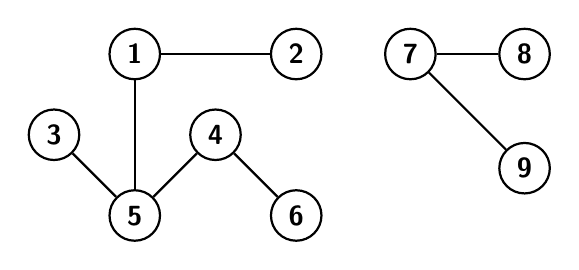
\begin{tikzpicture}[
    node distance=1.45cm, thick,
    main node/.style={circle, draw, font=\sffamily\bfseries}
]
    \node[main node] (1)                    {1};
    \node[main node] (3) [below left  of=1] {3};
    \node[main node] (4) [below right of=1] {4};
    \node[main node] (2) [above right of=4] {2};
    \node[main node] (5) [below right of=3] {5};
    \node[main node] (6) [below right of=4] {6};
    \node[main node] (7) [right of=2] {7};
    \node[main node] (8) [right of=7] {8};
    \node[main node] (9) [below of=8] {9};

    \path (1) edge (2)
        (1) edge (5)
        (3) edge (5)
        (4) edge (5)
        (4) edge (6)
        (7) edge (8)
        (7) edge (9);
\end{tikzpicture}
\caption{En skog}
\end{figure}
\end{column}
\end{columns}
\end{frame}

\begin{frame}{Rotfestede trær}
    \begin{itemize}
        \item Et \emph{rotfestet} tre er et tre med en dedikert rotnode.
        \item Nodene 'under' en annen node kalles for \emph{barnene} til noden.
        \item Noden 'over' en node kalles for forelderen. Alle unntatt roten har en forelder.
        \item Et binærtre er et rotfestet tre der alle har enten 0, 1 eller 2 barn.
    \end{itemize}
    \begin{columns}
    \begin{column}{0.48\textwidth}
\begin{figure}
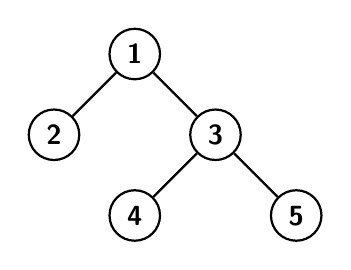
\begin{tikzpicture}[
    node distance=1.45cm, thick,
    main node/.style={circle, draw, font=\sffamily\bfseries}
]
    \node[main node] (1)                    {1};
    \node[main node] (2) [below left  of=1] {2};
    \node[main node] (3) [below right of=1] {3};
    \node[main node] (4) [below left of=3] {4};
    \node[main node] (5) [below right of=3] {5};

    \path (1) edge (2)
        (1) edge (3)
        (3) edge (4)
        (3) edge (5);
\end{tikzpicture}
\caption{binary tre}
\end{figure}
 \end{column}
    \begin{column}{0.48\textwidth}
\begin{figure}
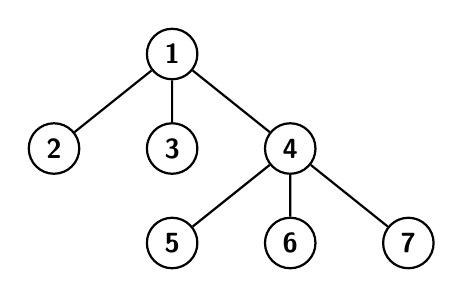
\begin{tikzpicture}[
    node distance=1.45cm, thick,
    main node/.style={circle, draw, font=\sffamily\bfseries},level distance=1.2cm,
  level 1/.style={sibling distance=1.5cm},
  level 2/.style={sibling distance=1.5cm}
]
  \node[main node] {1}
  	child {node[main node] {2}}
    child {node[main node] {3}}
    child {node[main node] {4}
    child {node[main node] {5}}
      child {node[main node] {6}}
    child {node[main node] {7}}
    };
\end{tikzpicture}
\caption{3-ary tre}
\end{figure}
\end{column}
\end{columns}
\end{frame}